\chapter{Development of the FPGA Firmware for the SFH}\label{cha:development}
\noindent
\section{Overview of the Firmware}
The firmware of the different FPGAs differs only by their port assignment, but otherwise are identical.
\newline
The firmware must perform several functionalities.
\newline
The main tasks of the firmware are to configure the Citiroc1A ASICs, explained in Section \ref{sec:configuration},
 communicaton with the controlling computer via Ethernet and the IPBUS protocol and a provisional readout of the time triggerd data from the Citiroc1A ASICs.
\newline
The firmware is written in VHSIC Hardware Description Language (VHDL) and is synthesized and implemented using Xilinx Vivado.
Several IP-cores, provided by Xilinx, are used to simplfy the development of the firmware for several tasks like the implementation of the configuration memory.
\subsection{The IPBUS Protocol}
The IPBUS protocol used for the communication between the FPGA and the controlling computer is a simple protocol for controlling IP-aware hardware devices with a 32 bit read and write bus using UDP as the transport protocol.\autocite{IPBUS_article}
\newline
The IPBUS protocol defines a read and write command enabling successful write and read operations of a 32 bit register, with a 32 bit address in the FPGA.    
\newline
The commands can be issued on the controling computer with the $\mu$HAL library, which allows the user to issue read and write commands using a python script and an XML file defining the addresses of the registers.\autocite{IPBUS_article}
\newline
The address space inside the FPGA is defined in the firmware. 
\subsection{The Firmware Structure}

\begin{figure}[H]
    \centering
    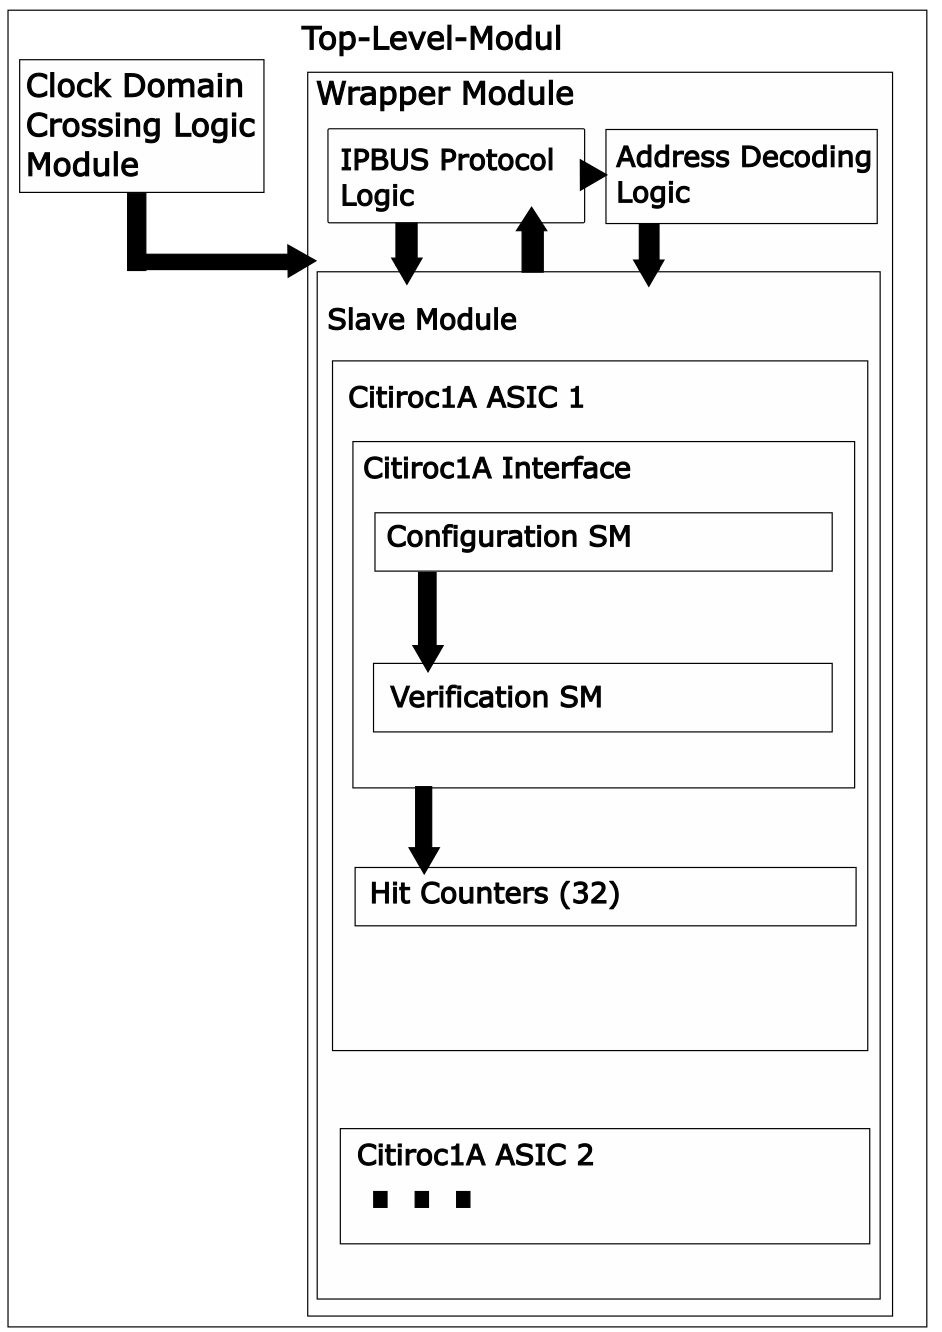
\includegraphics[width=0.75\textwidth]{Rastergrafik_mit_pfeile.png}%{E18Logo.png}%
    \caption{Hierarchical structure of the firmware, where each module contains its submodules.
    The black arrows indicate connections that are semantically correct but are routed through higher-level modules.}
    \label{fig:Firmware_structure}
\end{figure}

The firmware has a hierarchical structure illustrated in Figure \ref{fig:Firmware_structure}. 
\newline
The top level modul of the firmware defines the interconnections between internal FPGA logic and external components such as the Ethernet transceiver, clock oscillators and Citiroc1A ASICs.
\newline
The FPGA logic includes an IPBUS IP core and the slave entities in addition to a Clock Crossing Domain logic modul wich synchronizes the time triggerd Citiroc1A signals. 
\newline

The slave modul contains two identical Citiroc1A modules one for each ASIC, The Citiroc1A interface is instantiated for the configuration and verification of the ASIC.
The hitcounters allow to perform hit rate measurements for the 32 channels of the Citiroc1A ASIC. 
\section{The Address Space}
The 32 bit address is divided into sub addresses by the address decoding logic of the firmware.
\newline
The address space is first divided between the two Citiroc1A ASICs:
\begin{figure}[H]
    \centering
\begin{tabular}{p{7cm} l}
    \textbf{Citiroc1A Interface ASIC 1:} & 0000\_0000\_0000\_0000\_0\textcolor{red}{001}\_0000\_0000 \\
    \textbf{Citiroc1A Interface ASIC 2:} & 0000\_0000\_0000\_0000\_0\textcolor{red}{010}\_0000\_0000 \\
    \textbf{Hitcounters of ASIC 1:} & 0000\_0000\_0000\_0000\_0\textcolor{red}{011}\_0000\_0000 \\
    \textbf{Hitcounters of ASIC 2: } & 0000\_0000\_0000\_0000\_0\textcolor{red}{100}\_0000\_0000\\
\end{tabular}
\end{figure}

The address space of the Citiroc1A Interface is further divided into the following sub addresses:
\begin{figure}[H]
    \centering
\begin{tabular}{p{7cm} l}

     \textbf{Status and Control Register:} & 0000\_0000\_0000\_0000\_0000\_\textcolor{red}{00}00\_0000 \\
     \textbf{Configuration RAM:} & 0000\_0000\_0000\_0000\_0000\_\textcolor{red}{01}\textcolor{blue}{00\_0000} \\
     \textbf{Verification RAM:} & 0000\_0000\_0000\_0000\_0000\_\textcolor{red}{10}\textcolor{blue}{00\_0000}  \\ 
    
\end{tabular}
\end{figure}
In order to read the second address of the configuration RAM of the first Citiroc1A ASIC, the address would be:
\newline
0000\_0000\_0000\_0000\_0001\_0100\_0001
\newline
The address space of the hitcounters is also further divided into sub addresses:
\begin{figure}[H]
    \centering
 \begin{tabular}{p{7cm} l}
        \textbf{Hitcounter 0:} & 0000\_0000\_0000\_0000\_0000\_\textcolor{red}{00}0\textcolor{blue}{0\_0001} \\
        \textbf{Timecounter 0:} & 0000\_0000\_0000\_0000\_0000\_\textcolor{red}{01}0\textcolor{blue}{0\_0001} \\
        \textbf{Hitcounter 1:} & 0000\_0000\_0000\_0000\_0000\_\textcolor{red}{00}0\textcolor{blue}{0\_0010} \\
        \textbf{Timecounter 1:} & 0000\_0000\_0000\_0000\_0000\_\textcolor{red}{01}0\textcolor{blue}{0\_0010} \\
        \textbf{...} & ... \\
        \textbf{Hitcounter 31:} & 0000\_0000\_0000\_0000\_0000\_\textcolor{red}{00}0\textcolor{blue}{1\_1111} \\
        \textbf{Timecounter 31:} & 0000\_0000\_0000\_0000\_0000\_\textcolor{red}{01}0\textcolor{blue}{1\_1111} \\
 \end{tabular}
\end{figure}
The address to read the timecounter of the fifth channel of the second Citiroc1A ASIC would be:
\newline
0000\_0000\_0000\_0000\_0100\_0100\_0101

\section{Configuration of the Citiroc1A ASIC}

The configuration of the slow control and probe registers of the Citiroc1A ASIC,
along with the verification of this configuration, is handled by two finite state machines.
\newline
Each state machine controls a random access memory (RAM) with a depth of 64 addresses,
with each address storing 32 bits of data.
\newline
The state machiens in turn are controlled by the status and control register of the corresponding Citiroc1A Interface, which can be written by the controlling computer via the IPBUS protocol.
\subsection{Status and Control Register}
Each Citiroc1A interface has a 32 bit status and control register, but only the first 7 bits are used.
It is responsible for the control of the configuration and verification state machines as well as the hitcounters.
The bits of the status and control register, with the exception of bit 1
do not reset themselves after being set to 1 and have to be deaserted by the controlling computer.
\newline
Bit 1 is set to 0 by the FPGA after the configuration is loaded into the serial register.
\newline
Its structure is shown in Table \ref{tab:status_control_register}.
\begin{figure}[H]
    \centering
\begin{longtable}{|c|c|}
    \hline
    \textbf{Bit} & \textbf{Description} \\
    \hline
    \endfirsthead
    
    \hline
    \textbf{Bit} & \textbf{Description} \\
    \hline
    \endhead
    
    \hline
    \endfoot
    
    \hline
    \endlastfoot
    bit 0 & Selects between slow control (1) and probe register (0) \\
    bit 1 & Loads the the configuration into the serial register\\
    bit 2 & Resets the Configuration and Verification SM and the Configuration RAM \\
    bit 3 & Resets the  Citiroc1A serial register \\
    bit 4 & Loads the configuration into the slow control register \\
    bit 5 & Resets the hitcounters associated with the Citiroc1A \\
    bit 6 & Enables the hitcounters associated with the Citiroc1A \\
    \hline
    \end{longtable}
    \caption{Structure of the status and control register of the Citiroc1A interface. 
    The specified commands are executed when the bits are set to 1. }  
    \label{tab:status_control_register}
\end{figure}  
  
\subsection{Configuration State Machine}
\begin{figure}[H]
    \centering
    \includegraphics[width=\textwidth]{CONFIGSMALLdiagramfarbe2900.png}%{E18Logo.png}%
    \caption{Finite state machine for configuring the Citiroc1A ASIC.
    States associated with the same processes are highlighted using the same color.}
    \label{fig:Configuration_state_machine}
\end{figure}
The Configuration state machine, embedded  in the firmware as shown in Figure \ref{fig:Firmware_structure}, is responsible for configuring the slow control and probe registers of the Citiroc1A ASIC.
The state machine is controlled by the status and control register, which is written by the controlling computer via the IPBUS protocol.
It has four processes, whose states are shown in different colors in Figure \ref{fig:Configuration_state_machine}.
\newline
The \textbf{\textcolor{cyan}{write}} process is responsible for writing the configuration data to the configuration RAM.
32 bits can be written to a specified address in the configuration ram at a time by the controlling computer.
\newline
The \textbf{\textcolor{yellow!60!black}{read}} process allows the controlling computer to read the content of the configuration RAM at the specified address.
\newline
The \textbf{\textcolor{red}{reset}} process resets the configuration RAM and the Configuration state machine and is initiated by setting bit 2 of the status and control register to 1.
\newline
The \textbf{\textcolor{VioletRed}{load}} process loads the configuration data from the configuration RAM into the serial register of the Citiroc1A ASIC. 
The first 1144/256 bits of the configuration RAM are shifted into the serial register of the Citiroc1A ASIC, depending on the selected register.
Each bit is shifted in by setting the data line \textbf{\textcolor{red}{Srin\_sr}} and clock \textbf{\textcolor{red}{clk}} as described in Section \ref{sec:configuration}.
Since as discribed in Section \ref{sec:configuration} the first bit written to the serial register is the last bit of the configuration, the controling computer has to write the bitstream in reverse order to the configuration RAM.
\newline
The \textbf{\textcolor{red}{clk}} clock signal for thr ASIC's serial register is generated by the FPGA with a frequency of \SI{1}{\mega\hertz}.
The \textbf{\textcolor{VioletRed}{load}} process modulates this clock signal to control the operation of the serial register.
\newline
The process is repeated until all the data is shifted in and the configuration is loaded.
It can be initiated by the controlling computer by setting bit 1 of the status and control register to 1 and is only interruptible by the \textbf{\textcolor{red}{reset}} process.
\newline
In order to load the configuration into the slow control register from the serial register, bit 4 of the status and control register must be set to 1, this is not neccessary for the probe register.

\subsection{Verification State Machine}
\begin{figure}[H]
    \centering
    \includegraphics[width=\textwidth]{smallVerifacationdiagrammodfarbe.png}%{E18Logo.png}%
    \caption{Finite state machine for verifying the configuration of the Citiroc1A ASIC.
    States belonging to the same processes are represented with the same color.}
    \label{fig:Verification_state_machine}
\end{figure}
The Verification state machine, illustrated in Figure \ref{fig:Verification_state_machine} is responsible for verifying the configuration of the Citiroc1A ASIC.
It is incorporated into the firmware, as shown in Figure \ref{fig:Firmware_structure}.
\newline
It can be reset by the controling computer by setting bit 2 of the status and control register to 1.
\newline
If bits are shifted into the serial register of the Citiroc1A ASIC, the \textbf{\textcolor{green}{verification}} process is automatically started.
The \textbf{\textcolor{red}{srout}} signal coming back from the ASIC, explained in Section \ref{sec:configuration}, is used to read back the shifted bits from the serial register of the Citiroc1A ASIC.
The bits arrive at the FPGA in the same order as they were loaded in, but shifted by the length of the bitstream(1144/256). To compare the read back bits with the the loaded bits the bitstream has to be loaded twice.
\newline
The readback bits are stored in the verification RAM by the \textbf{\textcolor{green}{verification}} process and can be read by the controling computer via the  \textbf{\textcolor{yellow!60!black}{read}} process.
This allowes the controling computer to compare the loaded bits with the read back bits and ensure that the configuration was loaded correctly into the serial register of the Citiroc1A ASIC.
\section{The Provisional Readout}
In addition to the configuration and verification of the configuration of Citiroc1A ASIC, the firmware also provides a provisional readout in form of hitcounters and timecounters. 
\newline
The hitcounters are used to count the number of hits on each channel of the Citiroc1A ASIC.
\newline
They are limited to a minimal time between hits of two periods of the synchronization clock.
In this case a \SI{325}{\mega\hertz} clock is used, which corresponds to a minimal time between hits of \SI{6.16}{\nano\second}.
\newline
Each Citiroc1A has 32 hitcounters, one for each channel.
The 32 bit hitcounters are enabled by setting bit 6 of the status and control register of the corresponding Citiroc1A Interface to 1. 
This also enables the timecounter, which counts the number of clock cycles since it was last reset. 
\newline
The hitcounters and timecounters are reset by setting bit 5 of the status and control register of the corresponding Citiroc1A Interface to 1.
\newline
To read the hit and time counters, the controling computer first has to disable the hitcounters by setting bit 6 of the status and control register to 0, in order to avoid metastability issues arising from the clock domain crossing.
The hitcounters can then be read by the controlling computer via the IPBUS protocol.
\newline
The combination of the hitcounters and the timecounter allows the controlling computer to determine the number of hits per second on each channel of the Citiroc1A ASIC. 


\section{Testing the Firmware}
\subsection{Setup for the Noise Measurment}
The firmware will be evaluated through a noise measurement of the frontend electronics of the scintillating fiber hodoscope. 
The measurement will be performed with the SiPMs disconnected from the frontend electronics. 
The experimental setup is illustrated in Figure \ref{fig:noise_setup}.
\begin{figure}[H]
    \centering
    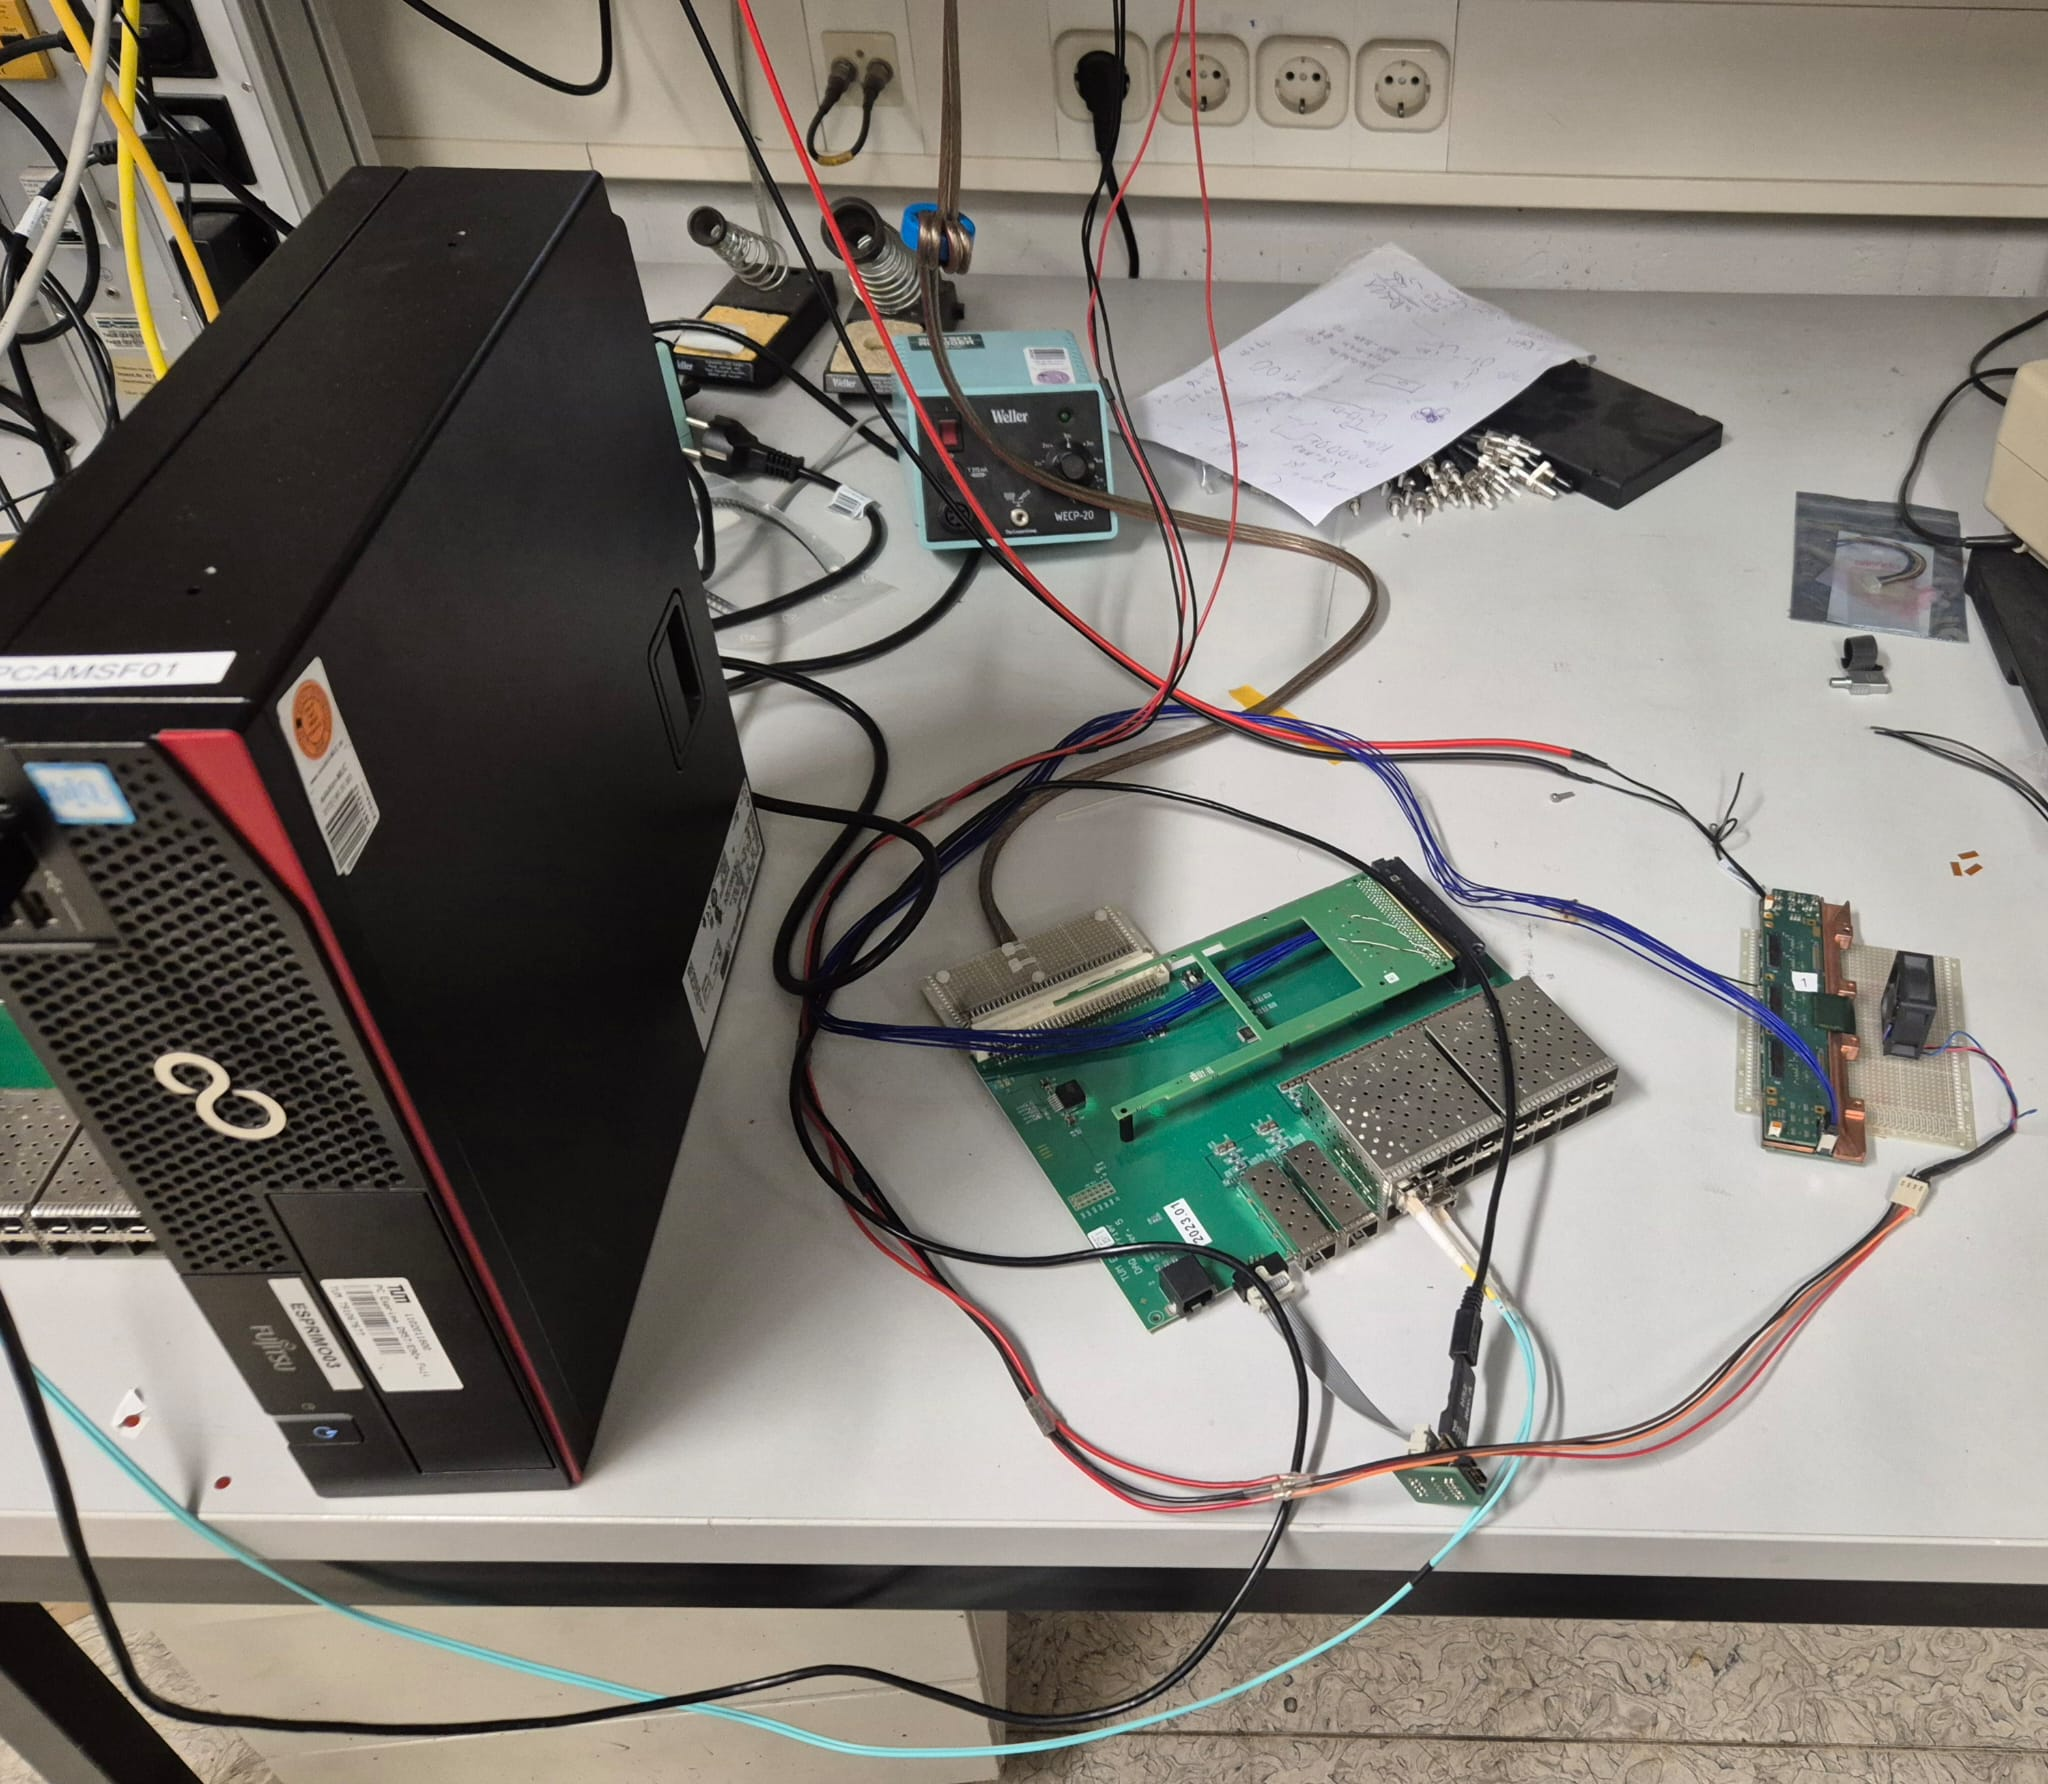
\includegraphics[width=0.8\textwidth]{WhatsApp Bild 2024-12-05 um 16.27.30_2637fa81.jpg}%{noise_setup.png}%{E18Logo.png}%
    \caption{Experimental setup for the noise measurement of the frontend electronics of the scintillating fiber hodoscope.}
    \label{fig:noise_setup}
\end{figure}
The measurement will be performed by the controlling computer, 
which will scan through a range of thresholds of the time discriminator of the Citiroc1A ASIC and record the number of hits per second on each channel with a measurement time of \SI{400}{\milli\second}.
This scan will be performed for several different high gains near the maximum value of 62.
\newline
For comparison, the threshold scan will also be performed with the same configuration of the Citiroc1A ASICs on an Evaluation Board provided by Weeroc company, 
with the setup shown in Figure \ref{fig:noise_setup_testboard}.
\begin{figure}[H]
    \centering
    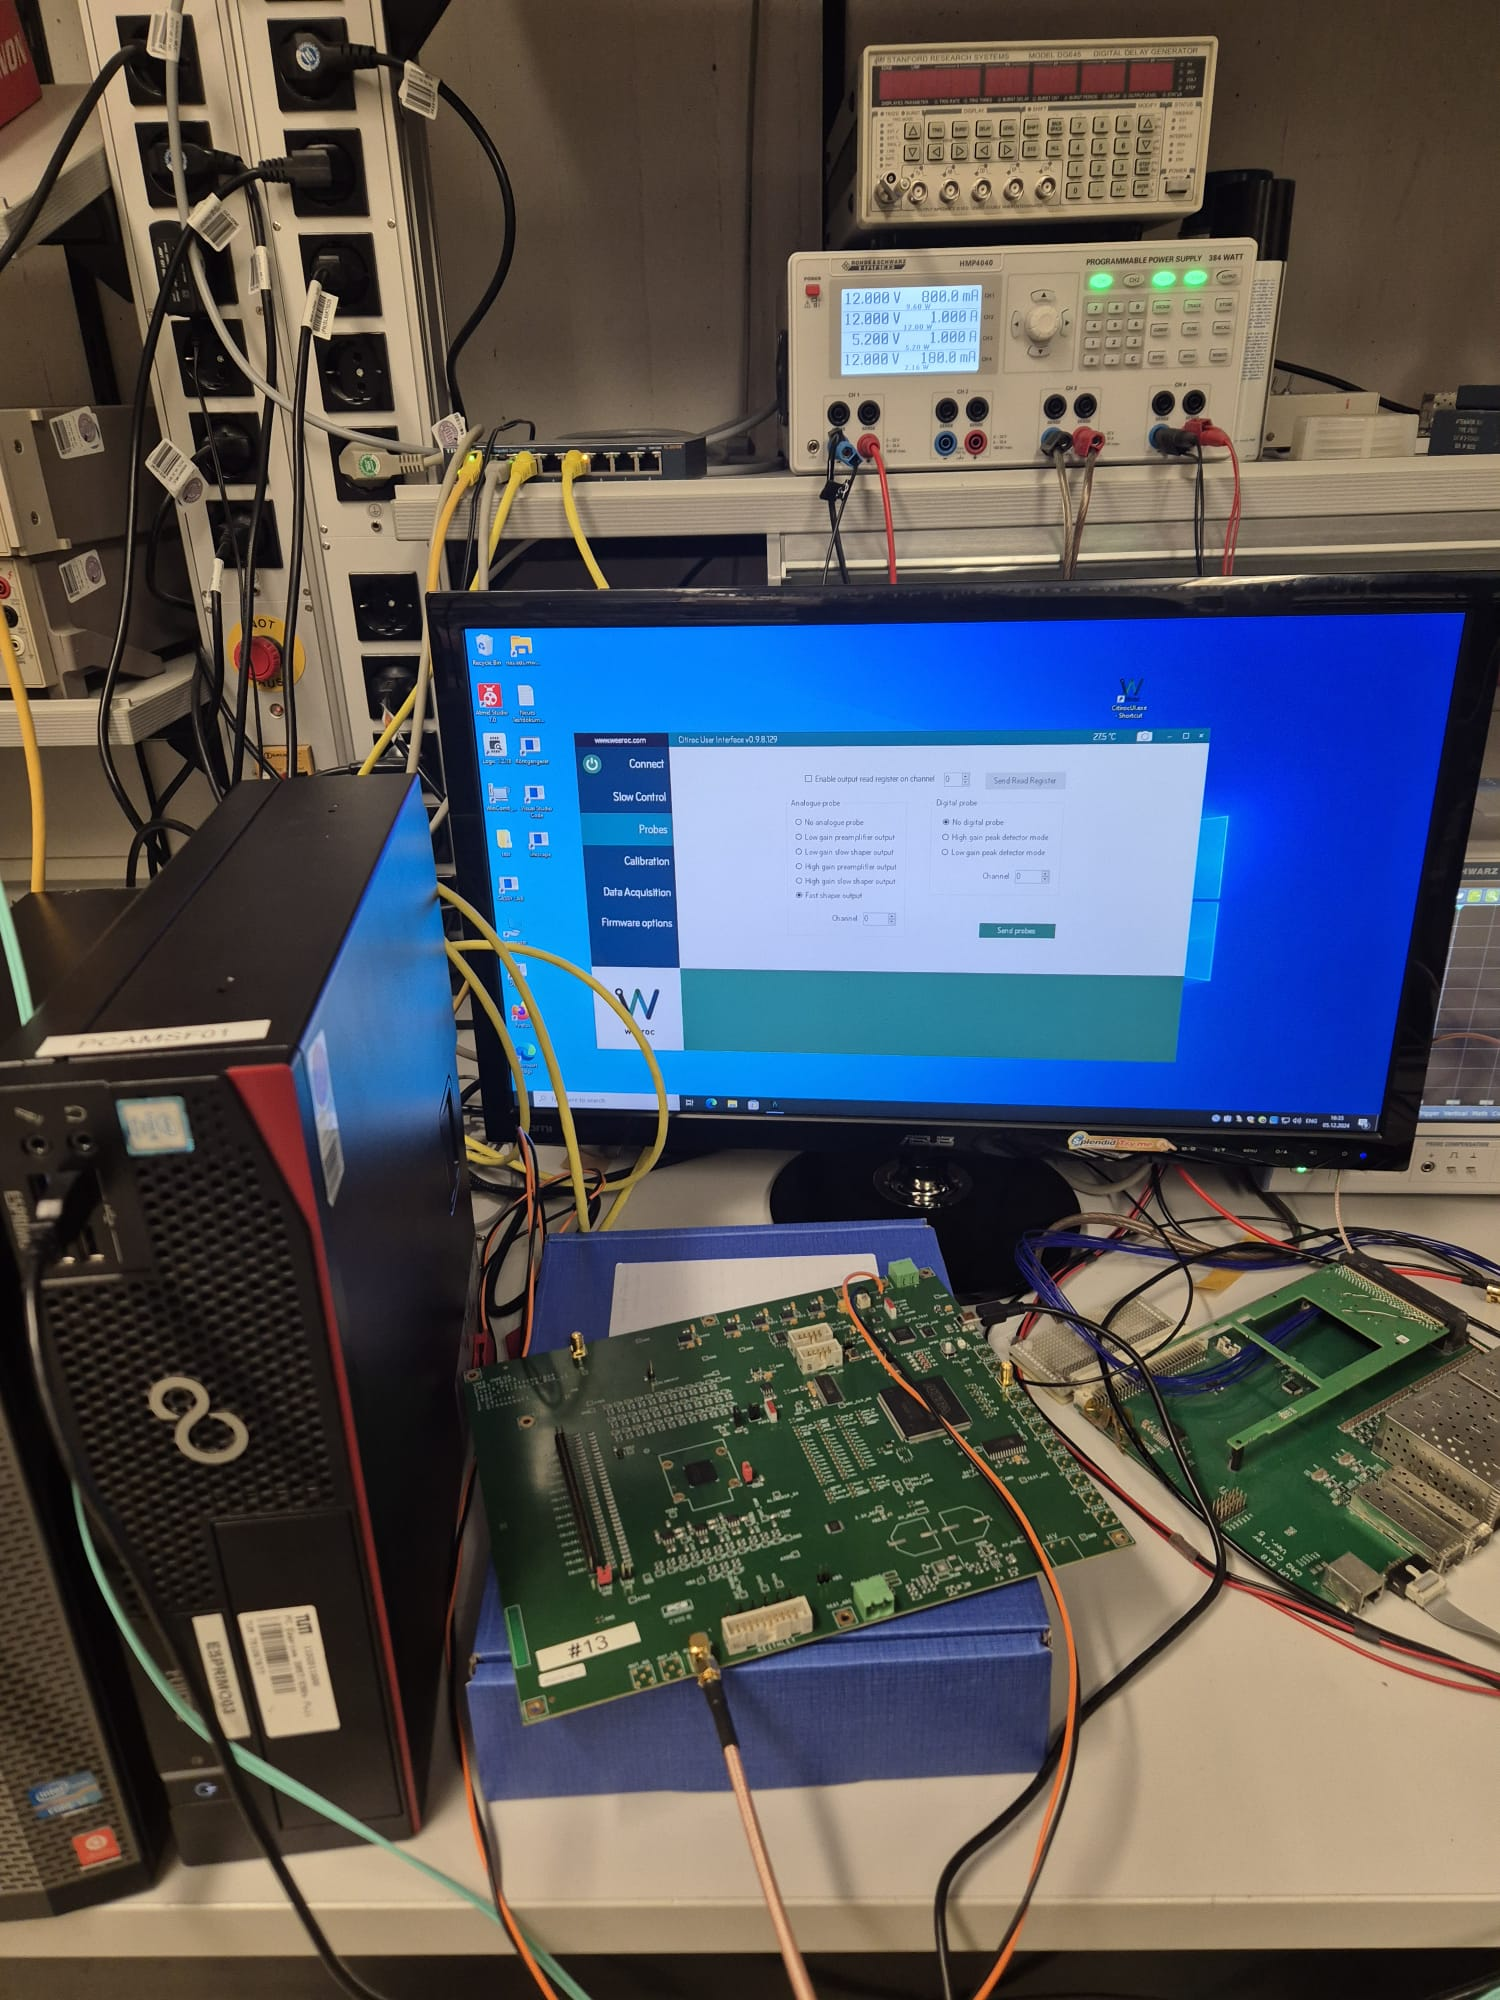
\includegraphics[width=0.8\textwidth]{WhatsApp Bild 2024-12-05 um 16.35.49_ef329d4e.jpg}%{noise_setup_testboard.png}%{E18Logo.png}%
    \caption{Experimental setup for the noise measurment with an Evaluation Board provided by Weeroc company.}
    \label{fig:noise_setup_testboard}
\end{figure}

\subsection{Theoretical Backround for the Noise Measurment} \label{sec:noise_theory}
The noise on the unconnected frontend electronics is assumed to be of gaussian distribution,
\begin{equation}
    P(x) = \frac{1}{\sqrt{2\pi}\sigma}e^{-\frac{(x-\mu)^2}{2\sigma^2}}
\end{equation}
where $\mu$ is the mean and $\sigma$ the standard deviation of the noise.\autocite{Theorynoise}
\newline
The number of hits per second on each channel of the ASIC is proportional to the number of noise events above the threshold of the time discriminator, but limited by the bandwidth of the fast shaper.\autocite{Theorynoise}
\newline
The number of hits per second vs the threshold of the time discriminator is expected to follow an S-curve, which can be described by a modified error function,
\begin{equation}
    N = \frac{A}{2} \left( 1 - \text{erf} \left( \frac{x - \mu}{\sqrt{2}\sigma} \right) \right)
\end{equation}
where $N$ is the number of hits per second, $x$ the threshold of the time discriminator and A an renormalization factor.\autocite{Theorynoise}